\documentclass{beamer}

% colors
\newcommand{\red}{\color{red!80!black}}
\newcommand{\blue}{\color{blue!90!black}}
\newcommand{\green}{\color{green!80!black}}
\newcommand{\purple}{\color{purple}}

% math commands
\usepackage{physics,bm}
\newcommand{\Ge}{\geqslant}
\newcommand{\Le}{\leqslant}
\newcommand{\ep}{\varepsilon}
\newcommand{\vp}{\varphi}
\newcommand{\avg}[1]{{\langle{#1}\rangle}}
\renewcommand{\d}{\text{d}}
\newcommand{\Prec}{\preccurlyeq}
\newcommand{\Succ}{\succcurlyeq}

% KLXX commands
\newcommand{\D}{\mathrm{d}}
\newcommand{\KL}{\mathrm{KL}}
\newcommand{\X}{\mathrm{X}}
\newcommand{\ESS}{\mathrm{ESS}}

\usepackage{algorithm2e}

% use the Madrid beamer theme
\mode<presentation> {
\usetheme{Madrid}
}
\usefonttheme{serif}
% keep beamer from re-declaring math alphabets over newtxmath (16-family limit)
\usefonttheme{professionalfonts}
\useinnertheme{circles}
\usepackage{caption}
\usepackage{tcolorbox}
% Times new Roman font
\usepackage{newtxtext,newtxmath}


% [] used in the footer, {} used in the title
\title[Mode Coverage via Log-Ratio Variation]{Mode Coverage in Boltzmann Generators\\ via Log-Ratio Variation}

\author[Xuda Ye]{Xuda Ye (Purdue)\\[6pt]
\small
Joint work with Qi Feng, Rongjie Lai and Di Qi}

\date[September 9, 2026]{September 9, 2026\\[6pt]
\small
Mathematics of Dynamical Systems in Modern Machine Learning\\
Brin Mathematics Research Center, UMD}


\begin{document}

\begin{frame}
	\titlepage
\end{frame}

\begin{frame}{The Sampling Problem, and Where It Fails}
	\small
	\begin{itemize}
		\setlength{\itemsep}{0pt}
		\item Given a potential $U$ on $\mathbb R^d$, draw samples from
		\begin{equation*}
			\pi(x)\propto e^{-U(x)} ,
		\end{equation*}
		with access to $U$ and $\nabla U$ alone.
		\item $U$ is multimodal: the mass splits among basins separated by barriers, and the quantity wanted is a ratio of masses between basins.
		\item {\red Mode collapse}: the sampler occupies some basins and never reaches the rest. Nothing it reports shows the absence.
	\end{itemize}
	\begin{center}
		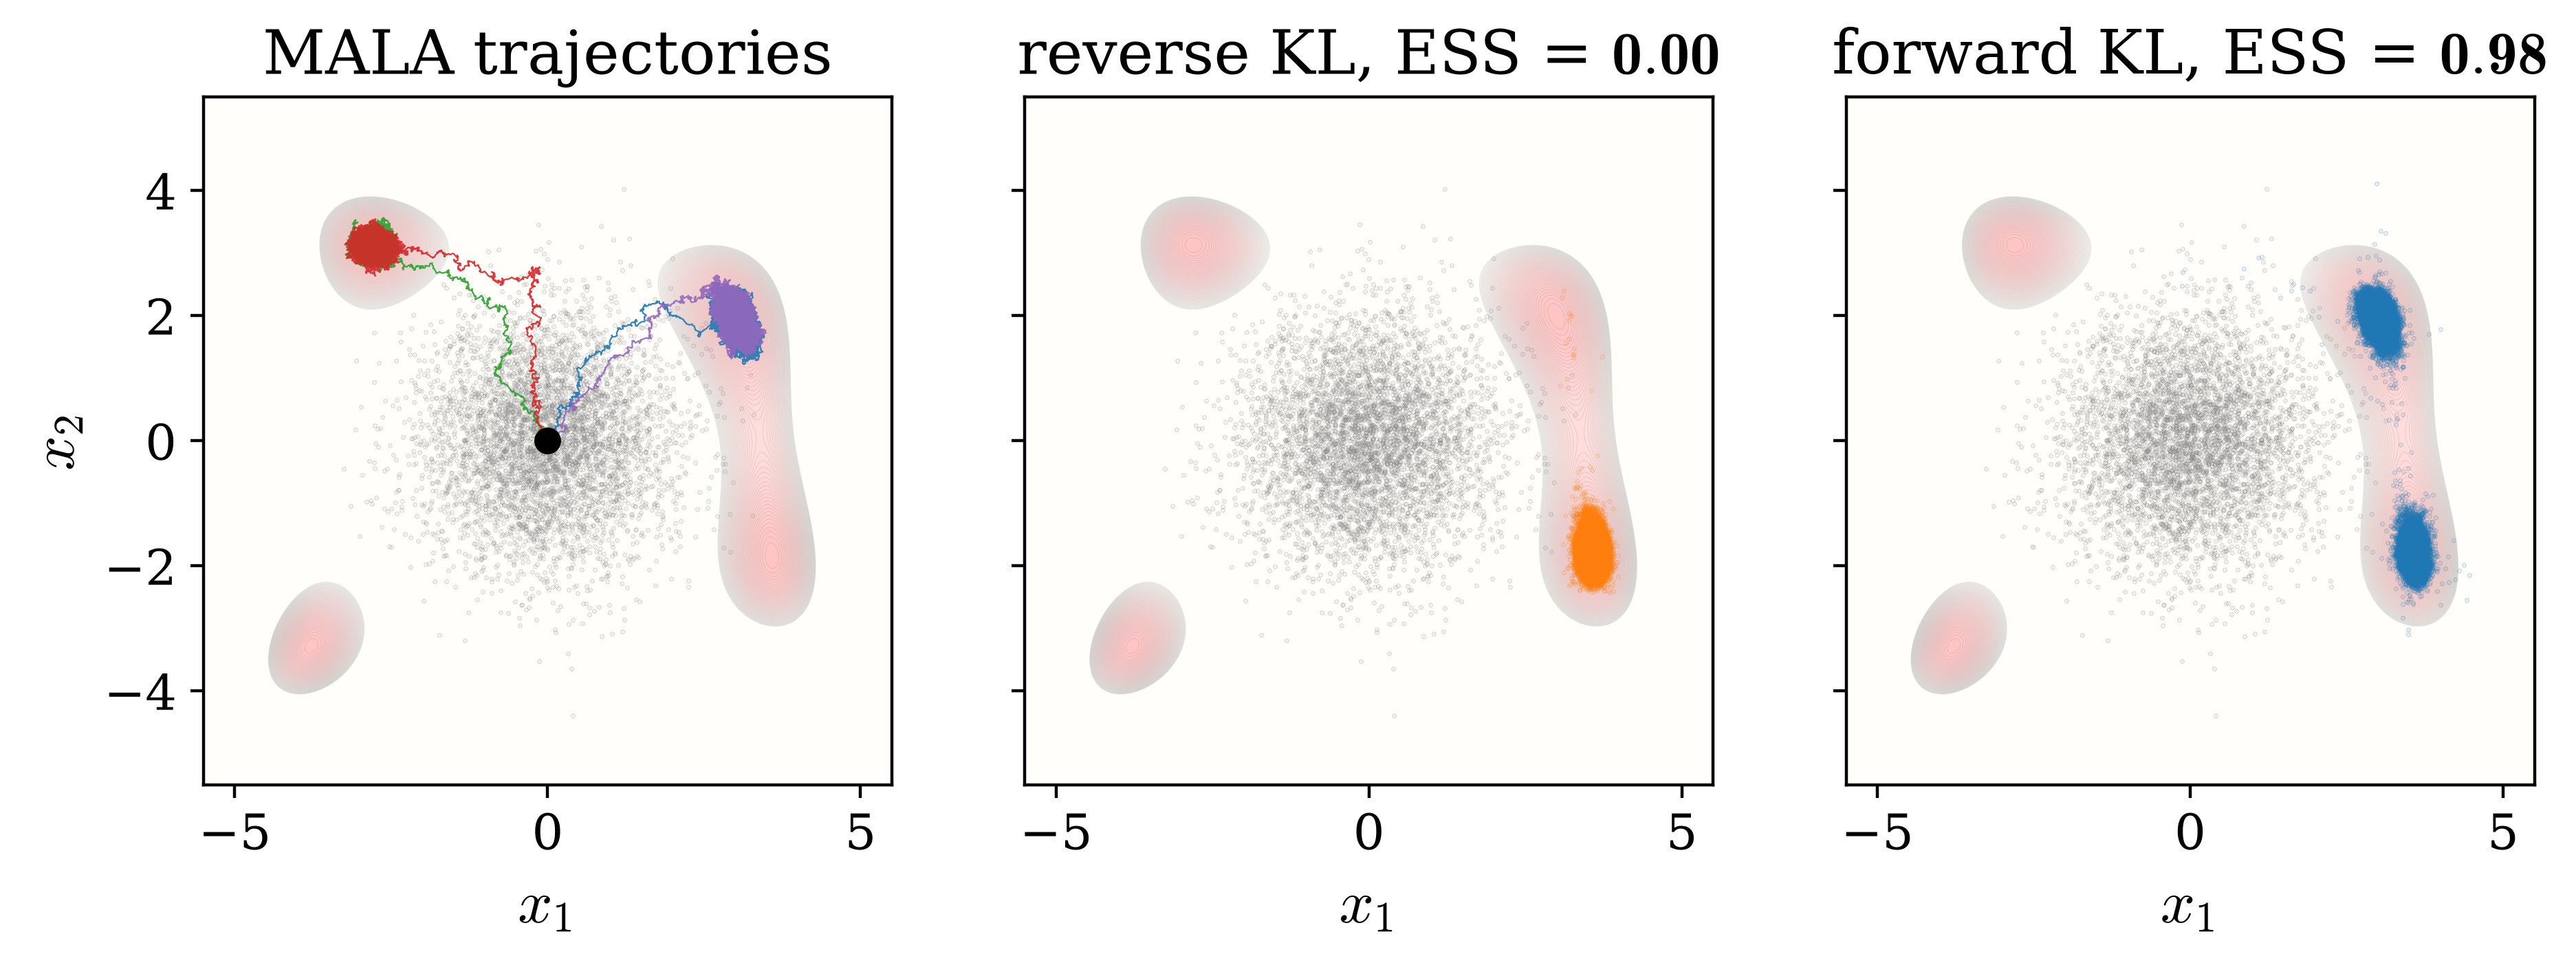
\includegraphics[width=0.9\textwidth]{figures/himmelblau_collapse.png}
	\end{center}
\end{frame}

\begin{frame}{Boltzmann Generators: a Global Transport}
	\small
	One invertible map in place of a Monte Carlo chain. [No\'e et al., \textit{Science} 2019]
	\begin{itemize}
		\setlength{\itemsep}{6pt}
		\item Source $\pi_0\propto e^{-U_0}$, Gaussian. Normalizing flow $G$ trained so that $G_{\#}\pi\approx\pi_0$.
		\item Pushforward $\nu:=(G^{-1})_{\#}\pi_0$, tractable density $\nu(y)=\pi_0(G(y))\bigl|\det J_G(y)\bigr|$.
		\item Conventional losses: reverse and forward KL,
		\begin{align*}
			\text{(reverse)}~~~ \KL(\nu\|\pi) & = \int_{\mathbb R^d} \nu(y) \log \frac{\nu(y)}{\pi(y)} \D y, \\
			\text{(forward)}~~~ \KL(\pi\|\nu) & = \int_{\mathbb R^d} \pi(y) \log \frac{\pi(y)}{\nu(y)} \D y.
		\end{align*}
		\item Reverse KL: {\red silent} where $\nu$ misses a mode of $\pi$.
		\item Forward KL: needs Monte Carlo samples of $\pi$ to train, and inherits their error.
	\end{itemize}
\end{frame}

\begin{frame}{Forward KL Can Still Have Mode Collapse}
	\small
	\begin{itemize}
		\setlength{\itemsep}{5pt}
		\item Weight $w(y)=\pi(y)/\nu(y)$, log-ratio $z=\log w$:
		\begin{equation*}
			{\blue z(y)} = U_0(G(y)) - U(y) - \log\bigl|\det J_G(y)\bigr| ,
			\qquad \KL(\pi\|\nu) = \mathbb E_{y\sim\pi}\bigl[{\blue z(y)}\bigr] .
		\end{equation*}
		\item Effective sample size $\ESS(w)=(\sum_i w_i)^2/(N\sum_i w_i^2)$ does not guarantee mode coverage. It can be {\red fake}.
	\end{itemize}
	\begin{center}
		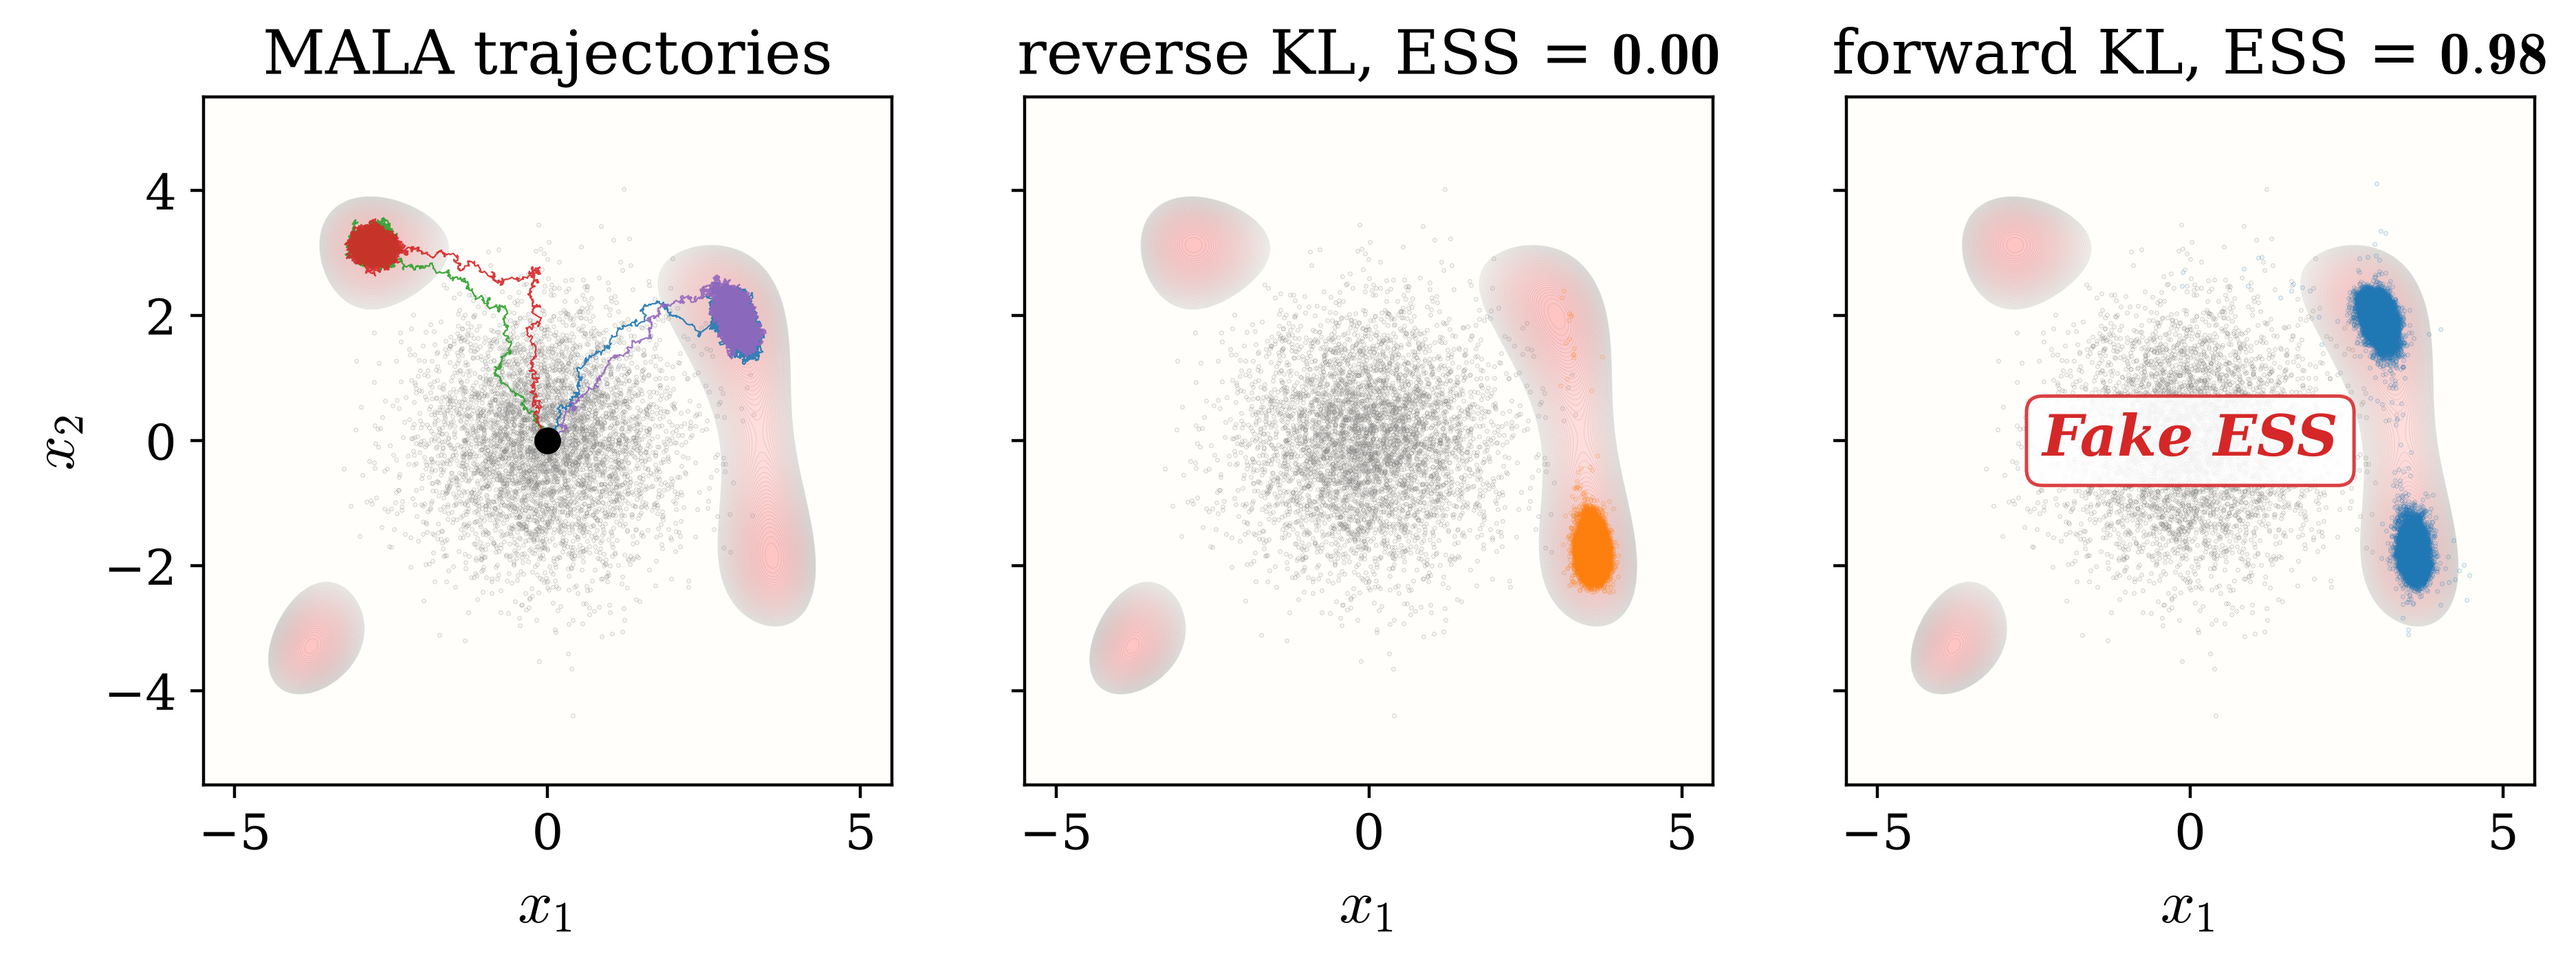
\includegraphics[width=0.9\textwidth]{figures/himmelblau_collapse_fake_ess.png}
	\end{center}
\end{frame}

\begin{frame}{The Log-Ratio Variation}
	\small
	Wanted: a term added to the forward KL. Evaluated at points from any distribution we can generate, needs {\blue no normalizing constant} of $\pi$, keeps $\nu=\pi$ a minimizer.
	\begin{block}{Log-ratio variation at a weighting distribution $\omega$}
		\begin{equation*}
			\X_\omega(\pi\|\nu)
			:= \mathbb E_{y,y'\sim\omega}\bigl[\,|z(y)-z(y')|\,\bigr],
			\qquad z = \log\frac{\pi}{\nu} .
		\end{equation*}
		Mean absolute pairwise difference of the log-ratio, both points drawn from $\omega$.
	\end{block}
	\begin{itemize}
		\setlength{\itemsep}{6pt}
		\item Normalizers cancel: a constant shift of $z$ leaves every difference unchanged.
		\item $\X_\omega(\pi\|\nu)=0$ exactly when $z$ is constant $\omega$-a.s., i.e.\ $\nu\propto\pi$.
		\item $\omega$ says where flatness is demanded, and {\red it need not be $\pi$}. That freedom is the whole design.
	\end{itemize}
\end{frame}

\begin{frame}{The KLXX Loss}
	\small
	Two log-ratio variations appended to the forward KL, the two X's:
	\begin{gather*}
		\mathrm{KLXX} [G] = \underbrace{\KL(\pi\|\nu)}_{\text{target fit}}
		+ \underbrace{\X_\pi(\pi\|\nu)}_{\text{\blue target variation}}
		+ \underbrace{\X_{(\hat\pi+\bar\nu)/2}(\pi\|\nu)}_{\text{\red mixture variation}} \\
		= \mathbb E_{y\sim\pi}\bigl[z(y)\bigr]
		+ \mathbb E_{y,y'\sim\pi}\bigl[|z(y)-z(y')|\bigr]
		+ \mathbb E_{y,y'\sim(\hat\pi+\bar\nu)/2}\bigl[|z(y)-z(y')|\bigr] .
	\end{gather*}
	\vspace{-0.5cm}
	\begin{itemize}
		\setlength{\itemsep}{4pt}
		\item $\hat\pi$: the quench and temper (QT) distribution, supplying candidate modes.
		\item $\bar\nu$: the detached pushforward, equal to $\nu$ but outside the differentiation graph.
	\end{itemize}
	\vspace{2pt}
	Generalized loss, mixture $\xi := \alpha\hat\pi+\beta\bar\nu$, with $\lambda,\vartheta,\alpha,\beta\Ge0$, $\alpha+\beta=1$:
	\begin{equation*}
		\mathcal L[G] = \KL(\pi\|\nu) + \lambda\,\X_\pi(\pi\|\nu) + \vartheta\,\X_{\alpha\hat\pi+\beta\bar\nu}(\pi\|\nu) .
	\end{equation*}
	{\red KLXX} is determined by $(\lambda,\vartheta,\alpha,\beta)=(1,1,\tfrac12,\tfrac12)$, written $\KL$+$\X_\pi$+$\X_{(\hat\pi+\bar\nu)/2}$.
\end{frame}

\begin{frame}{Quench and Temper: Finding Candidate Modes}
	\small
	Three steps on each source sample $y\sim\pi_0$. Oracle access to $U$ and $\nabla U$ only.
	\begin{enumerate}
		\setlength{\itemsep}{1pt}
		\item Melt: $y \gets y + m_e\zeta$, $\zeta\sim\mathcal N(0,I_d)$, at melt scale $m_e>0$.
		\item Quench: $\dot y = -\nabla U(y)$, into whichever basin the melted particle landed in.
		\item Temper: $\dot y = -\nabla U(y)+\sqrt2\,\dot B_t$, a spread around that basin.
	\end{enumerate}
	\begin{center}
		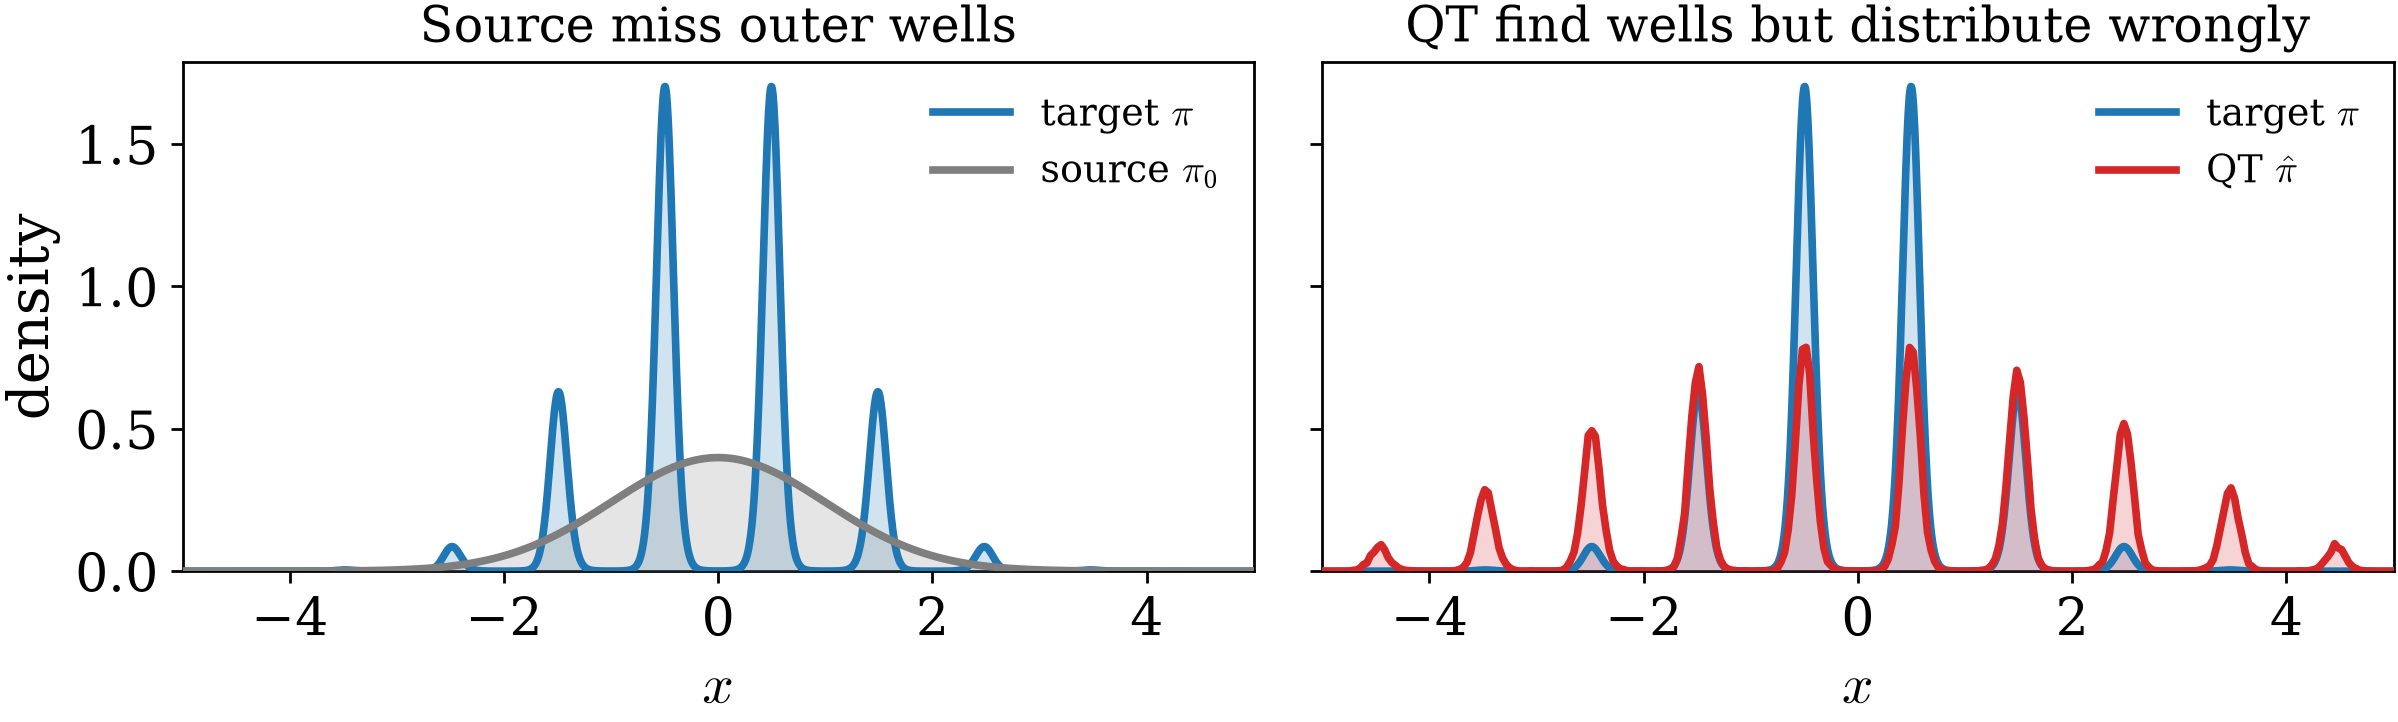
\includegraphics[width=\textwidth]{figures/1d_qt_density.png}
	\end{center}
\end{frame}

\begin{frame}{Why Mix QT with the Pushforward}
	\small
	\begin{itemize}
		\setlength{\itemsep}{3pt}
		\item $\hat\pi$ is inaccurate everywhere. Admissible: a variation asks for flatness of $z$, never for the mass at those points.
		\item $\X_{\hat\pi}$ weights points inside the basins only, and says nothing where $\nu$ puts mass and $\hat\pi$ does not: the {\red intermodal} regions.
	\end{itemize}
	\begin{center}
		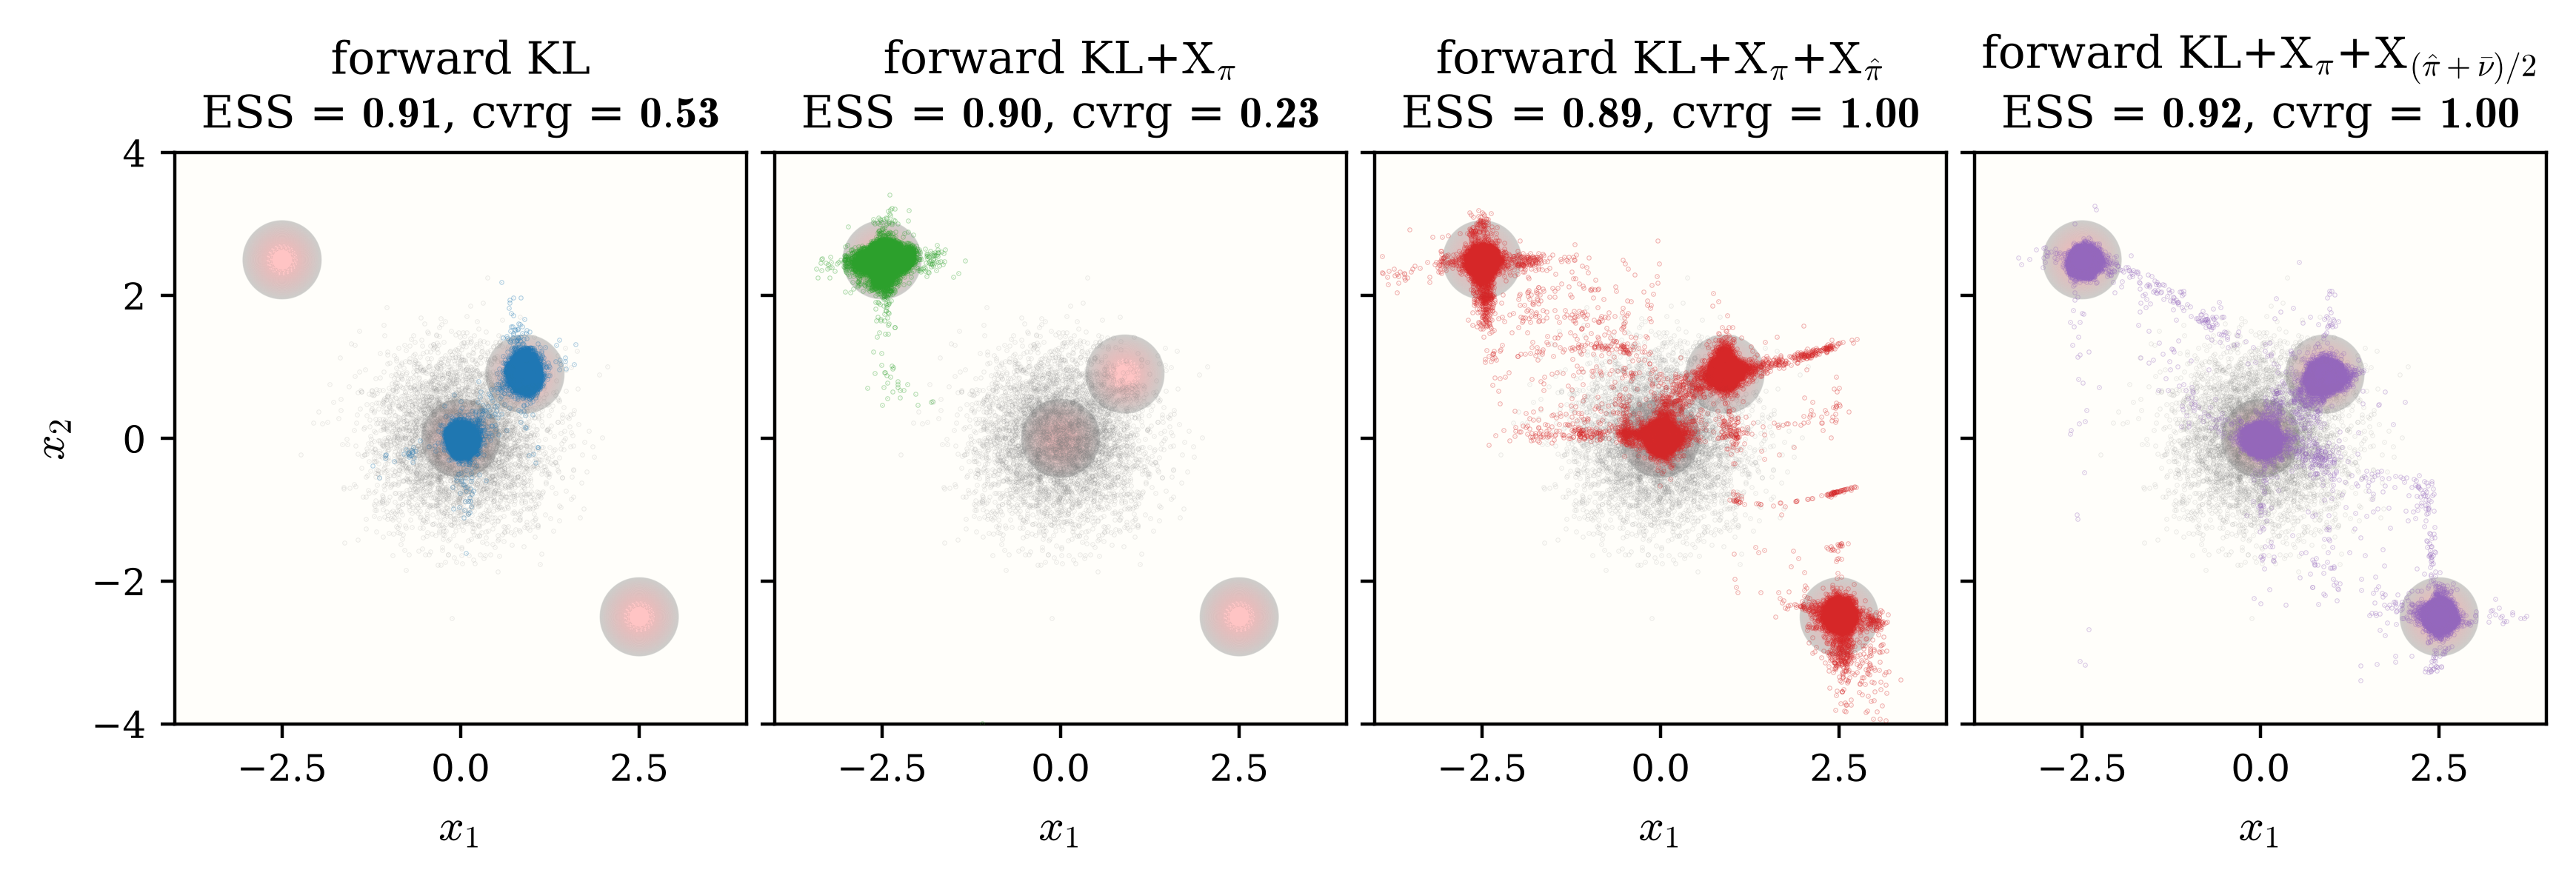
\includegraphics[width=\textwidth]{figures/2d_sparse_4methods.png}
	\end{center}
\end{frame}

\begin{frame}{The Collision: Why Mixture Handles Collapse?}
	Under the {\blue mixture} $\xi=\tfrac12(\hat\pi+\bar\nu)$, training drives
	\begin{equation*}
		z(y) \;=\; \log\frac{\pi(y)}{\nu(y)}
		\;\approx\;
		\log\frac{\pi(y')}{\nu(y')} \;=\; z(y') ,
		\qquad y\sim\hat\pi , \quad y'\sim\bar\nu .
	\end{equation*}
	\begin{itemize}
		\setlength{\itemsep}{9pt}
		\item $y$ in a target mode: $z(y)\to+\infty$ if $\nu$ {\red misses} it.
		\item $y'$ where the flow puts mass: $z(y')\to-\infty$ if $\nu$ {\red leaks}.
		\item Both hold only if $\nu$ covers every mode and avoids the intermodal regions.
	\end{itemize}
\end{frame}

\begin{frame}{KLXX Training Algorithm}
	\small
	Training of the generalized KLXX loss with parameters $(\lambda,\vartheta,\alpha,\beta)$.
	\begin{tcolorbox}[colback=gray!8,colframe=gray!45,boxrule=0.5pt,arc=2pt,
		left=6pt,right=6pt,top=5pt,bottom=5pt]
		Source samples $\mathcal Y_0\sim\pi_0$ and QT samples $\hat{\mathcal Y}=\mathrm{QT}(\mathcal Y_0,U)$, fixed before training.\\[4pt]
		Per gradient step, run:
		\begin{enumerate}
			\setlength{\itemsep}{3pt}
			\item pushforward batch $\mathcal X_\nu = G^{-1}(\mathcal X_0)$, from a random $\mathcal X_0\subset\mathcal Y_0$ of size $B$;
			\item target surrogate $\mathcal X_\pi = \mathrm{SMC}(\mathcal X_\nu)$, from pushforward $\nu$ to $\pi$;
			\item mixture batch $\mathcal X_\xi \sim \xi = \alpha\hat\pi + \beta\bar\nu$, drawn from $\hat{\mathcal Y}$ and $\mathcal X_\nu$.
		\end{enumerate}
		\vspace{2pt}
		\begin{equation*}
			\widehat{\mathcal L}[G]=\underbrace{\widehat{\mathbb E}_{y\in\mathcal X_\pi}\bigl[z(y)\bigr]}_{\text{forward KL}} +
			\lambda\underbrace{\widehat{\mathbb E}_{y,y'\in\mathcal X_\pi}\bigl[|z(y)-z(y')|\bigr]}_{\text{target variation}}
			+\vartheta\underbrace{\widehat{\mathbb E}_{y,y'\in\mathcal X_{\xi}}\bigl[|z(y)-z(y')|\bigr]}_{\text{mixture variation}}
		\end{equation*}
		One Adam step on $\widehat{\mathcal L}[G]$ updates $G$; only $z$ carries the gradient.
	\end{tcolorbox}
\end{frame}

% human review ends here

\begin{frame}{The Empirical Averages: Exact Calculation}
	\small
	\begin{itemize}
		\setlength{\itemsep}{5pt}
		\item On a batch $\mathcal X = \{y_1,\dots,y_B\}$, the empirical averages are
		\begin{align*}
			\widehat{\mathbb E}_{y\in\mathcal X}\bigl[z(y)\bigr]
			&:= \frac1B \sum_{i=1}^{B} z(y_i) ,
			\\[4pt]
			\widehat{\mathbb E}_{y,y'\in\mathcal X}\bigl[|z(y)-z(y')|\bigr]
			&:= \frac{2}{B(B-1)}\sum_{1\Le i<j\Le B} \bigl|z(y_i)-z(y_j)\bigr| .
		\end{align*}
		\item Each $z(y_i)$ is a scalar. Sorting $z_{(1)}\Le\cdots\Le z_{(B)}$ gives the double sum exactly,
		\begin{equation*}
			\sum_{i<j}\bigl|z(y_i)-z(y_j)\bigr| = \sum_{k=1}^{B}(2k-B-1)\,z_{(k)} ,
		\end{equation*}
		at cost {\red $O(B\log B)$}: the $\binom B2$ pairs are never formed.
	\end{itemize}
\end{frame}

\begin{frame}{Adaptive Staging Boltzmann Generator: Interpolation}
	\small
	One flow from $\pi_0$ to $\pi$ is not enough in high dimension. Interpolate the potentials and train one flow per {\blue stage}:
	\begin{equation*}
		U_t = (1-t)U_0 + tU , \qquad \pi_t \propto e^{-U_t} , \qquad
		0 = t_0 < t_1 < \cdots < t_K = 1 .
	\end{equation*}
	\vspace{-0.5cm}
	\begin{itemize}
		\setlength{\itemsep}{6pt}
		\item Stage $k$ carries $\pi_{k-1}\to\pi_k$, a deformation small enough for one flow.
		\item The schedule cannot be fixed in advance: no target data, no knowledge of where the wells are. The difficulty is unknown until it is attempted.
		\item {\red Accept a stage only when its sample ESS clears a gate $\tau_{\mathrm v}$}, otherwise shrink the increment and retry.
		\item Easy interpolations take large stages, hard ones take small.
	\end{itemize}
\end{frame}

\begin{frame}{Adaptive Staging Boltzmann Generator: Algorithm}
	\small
	\begin{tcolorbox}[colback=gray!8,colframe=gray!45,boxrule=0.5pt,arc=2pt,
		left=6pt,right=6pt,top=5pt,bottom=5pt]
		Sample set $\mathcal Y_0\sim\pi_0$, \ $t_0=0$. At the stage $t_{k-1}\mapsto t_k$:
		\begin{enumerate}
			\setlength{\itemsep}{4pt}
			\item propose $t_k$ by extrapolating the last accepted increment,
			$$
			t_k = \min\bigl(1,\ t_{k-1}+\Gamma(t_{k-1}-t_{k-2})\bigr);
			$$
			\item build the {\red QT set} $\hat{\mathcal Y}_k = \mathrm{QT}(\mathcal Y_{k-1},U_{t_k})$; \qquad {\blue (prebuilt before training)}
			\item train $G_k$ on $\pi_{k-1}\to\pi_k$ by the KLXX training algorithm using $\hat{\mathcal Y}_k$;
			\item weights $w_k = \exp(z_k)$ on $\mathcal Y_{k-1}$ pushed through $G_k^{-1}$.
			\\[4pt]
			If $\ESS(w_k)<\tau_{\mathrm v}$: shrink $t_k \gets t_{k-1}+\gamma\,(t_k-t_{k-1})$ and repeat from 2.
			\\[4pt]
			Otherwise: resample, rejuvenate under $U_{t_k}$, and set $\mathcal Y_k$.
		\end{enumerate}
	\end{tcolorbox}
	\vspace{2pt}
	Defaults $\tau_{\mathrm v}=0.4$, $\Gamma=1.5$, $\gamma=0.7$. Output: the schedule $\{t_k\}$ and the stage maps $\{G_k\}$, which the generator replays on fresh source samples.
\end{frame}

\begin{frame}{How the Error Propagates}
	\small
	Inference replays the accepted stages on $N$ fresh source particles: push forward, reweight, resample, rejuvenate.
	\begin{itemize}
		\setlength{\itemsep}{8pt}
		\item For every bounded observable $\varphi$, with $\pi_K^N$ the returned empirical measure, $w_k=\pi_k/\nu_k$ the stage weights and $\operatorname{osc}(\varphi)=\operatorname{ess\,sup}\varphi-\operatorname{ess\,inf}\varphi$,
		\begin{equation*}
			\bigl\lVert \pi_K^N\langle\varphi\rangle - \pi_K\langle\varphi\rangle \bigr\rVert_2
			\Le \frac{\operatorname{osc}(\varphi)}{2\sqrt N}
			\sum_{k=0}^{K}\ \prod_{j=k+1}^{K} 3\lVert w_j\rVert_\infty ,
		\end{equation*}
		\item {\red The scheme is asymptotically unbiased: its error is removed by raising $N$ alone.} Classical Monte Carlo instead needs the simulation time to grow.
	\end{itemize}
\end{frame}

\begin{frame}{2D Benchmarks: Three-Well and Himmelblau}
	\small
	\begin{center}
		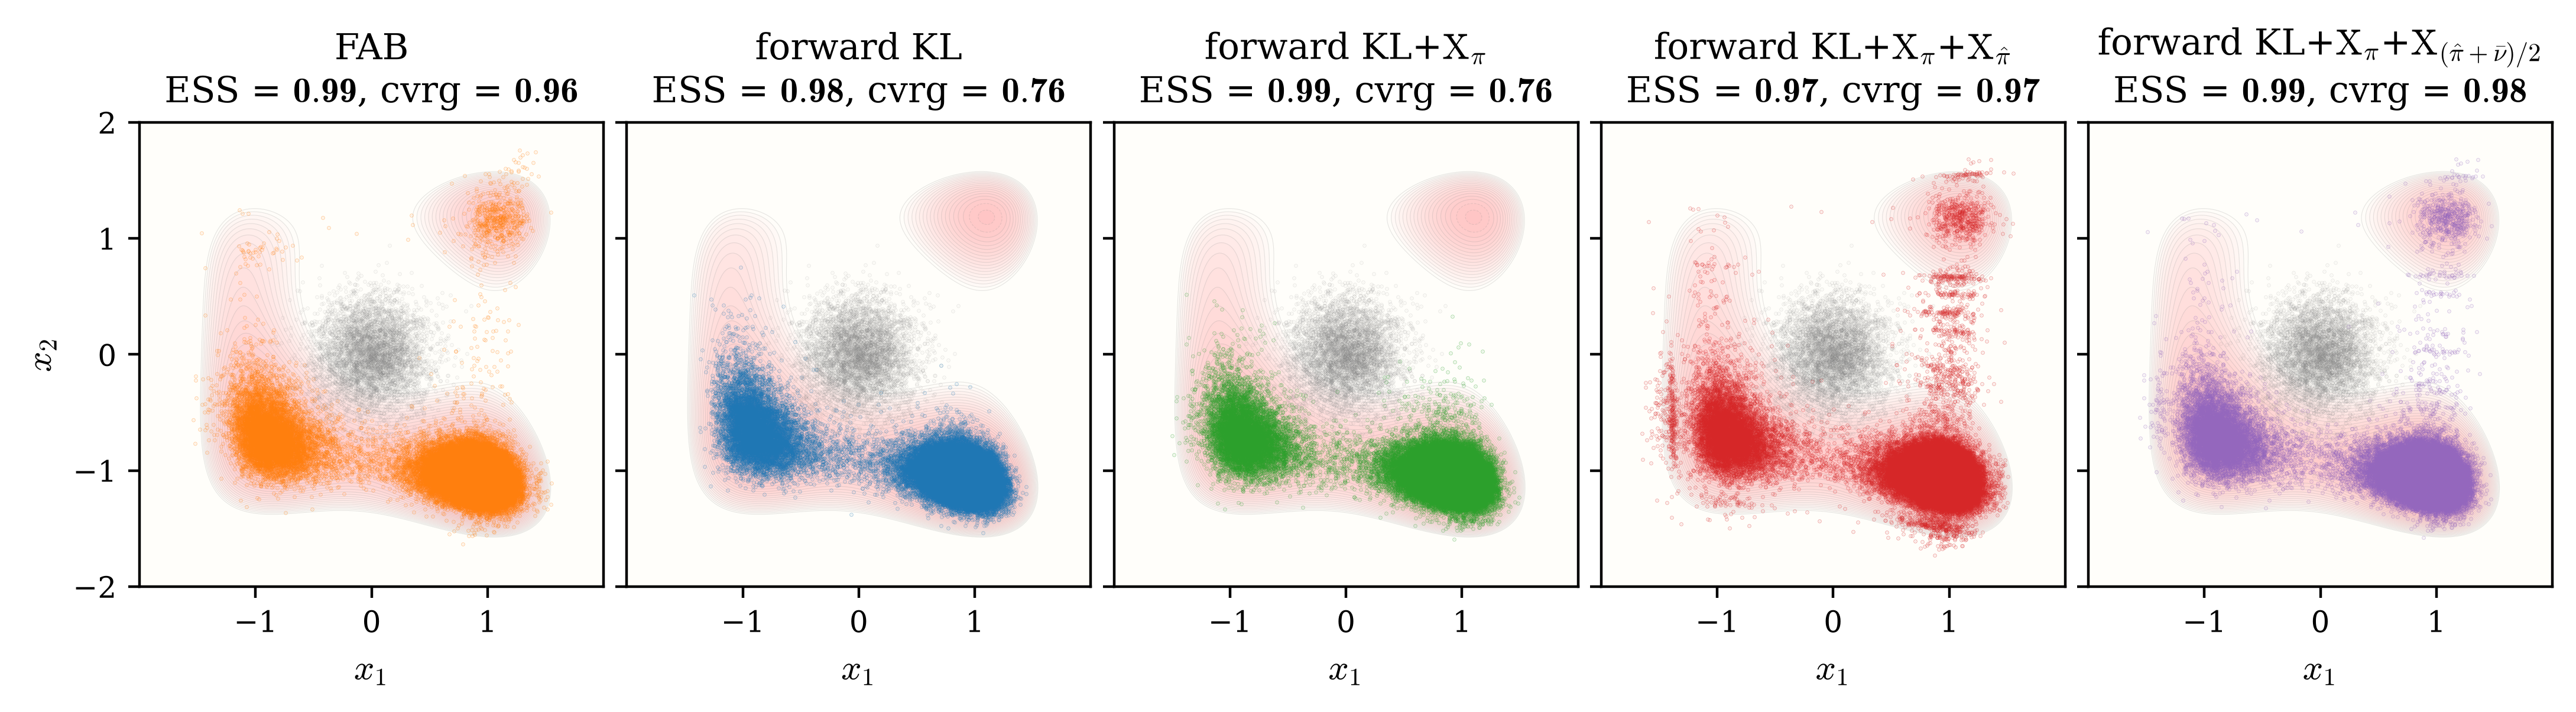
\includegraphics[width=\textwidth]{figures/2d_three_well_samples.png}\\[3pt]
		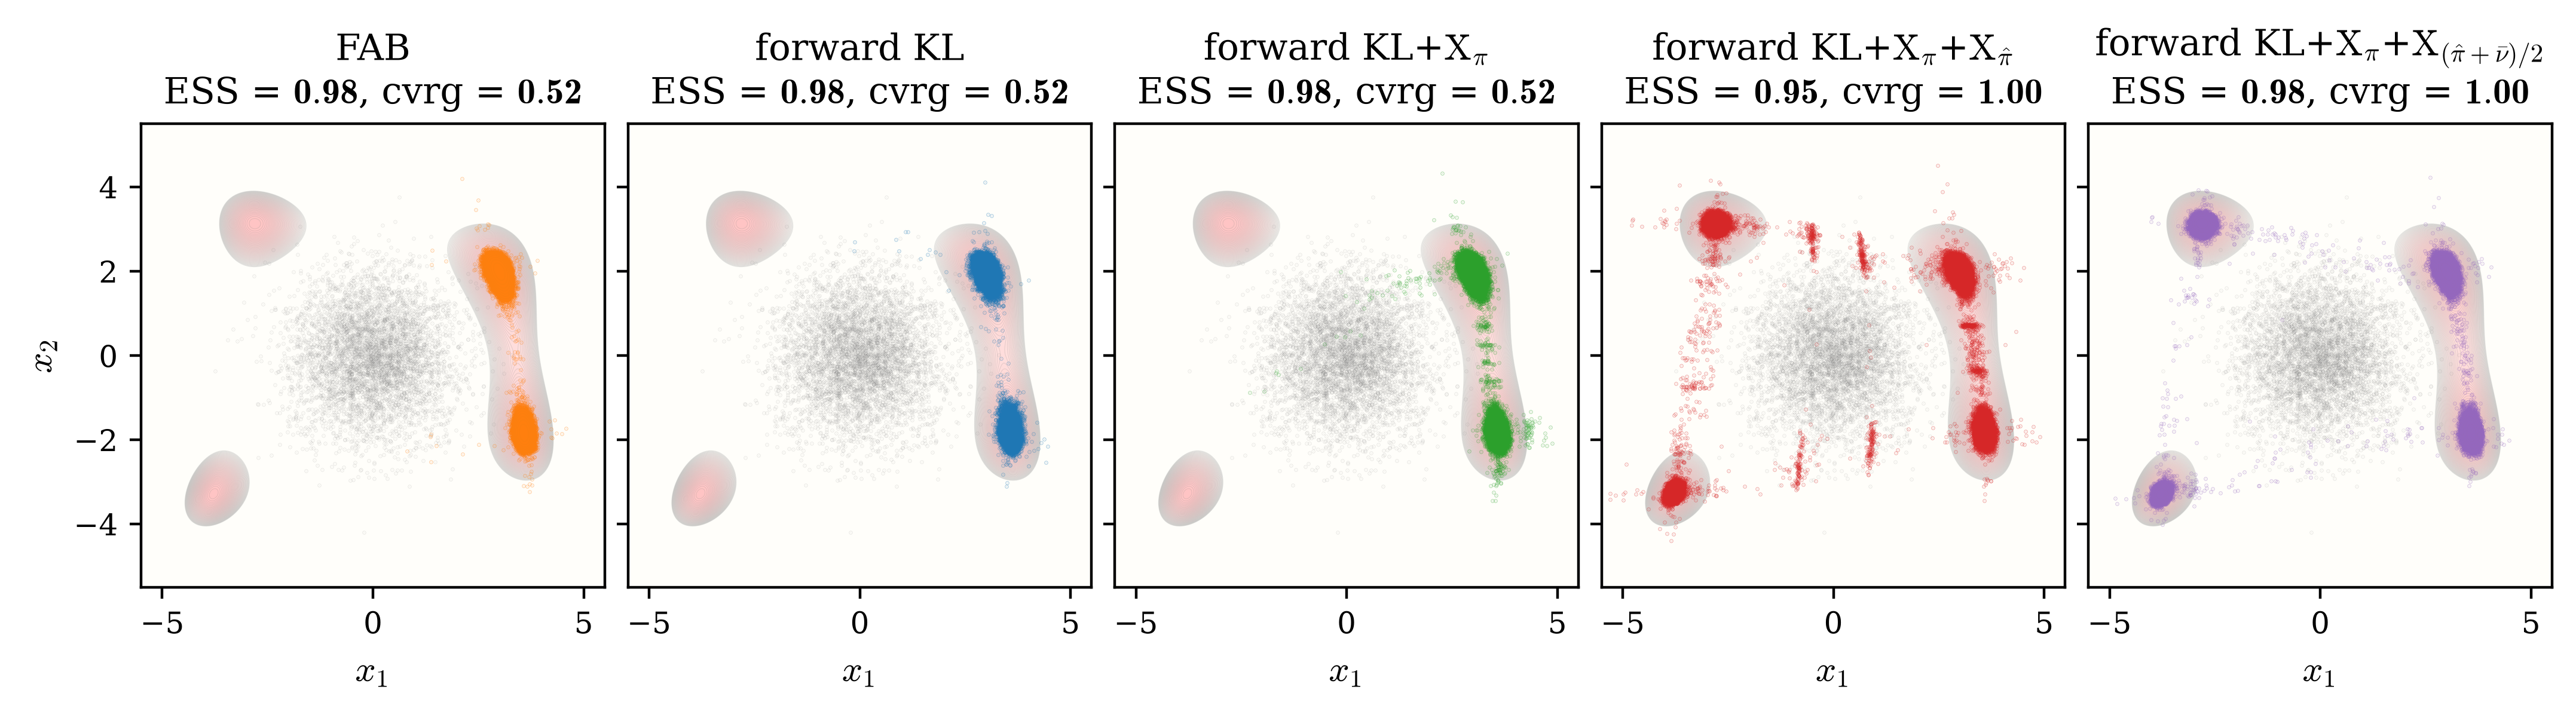
\includegraphics[width=\textwidth]{figures/2d_himmelblau_samples.png}
	\end{center}
	\vspace{-2pt}
	\centering
	Three-Well (top), Himmelblau (bottom). Every method reports a high ESS.
\end{frame}

\begin{frame}{2D Benchmarks: Where the ESS Is Earned}
	\small
	\begin{center}
		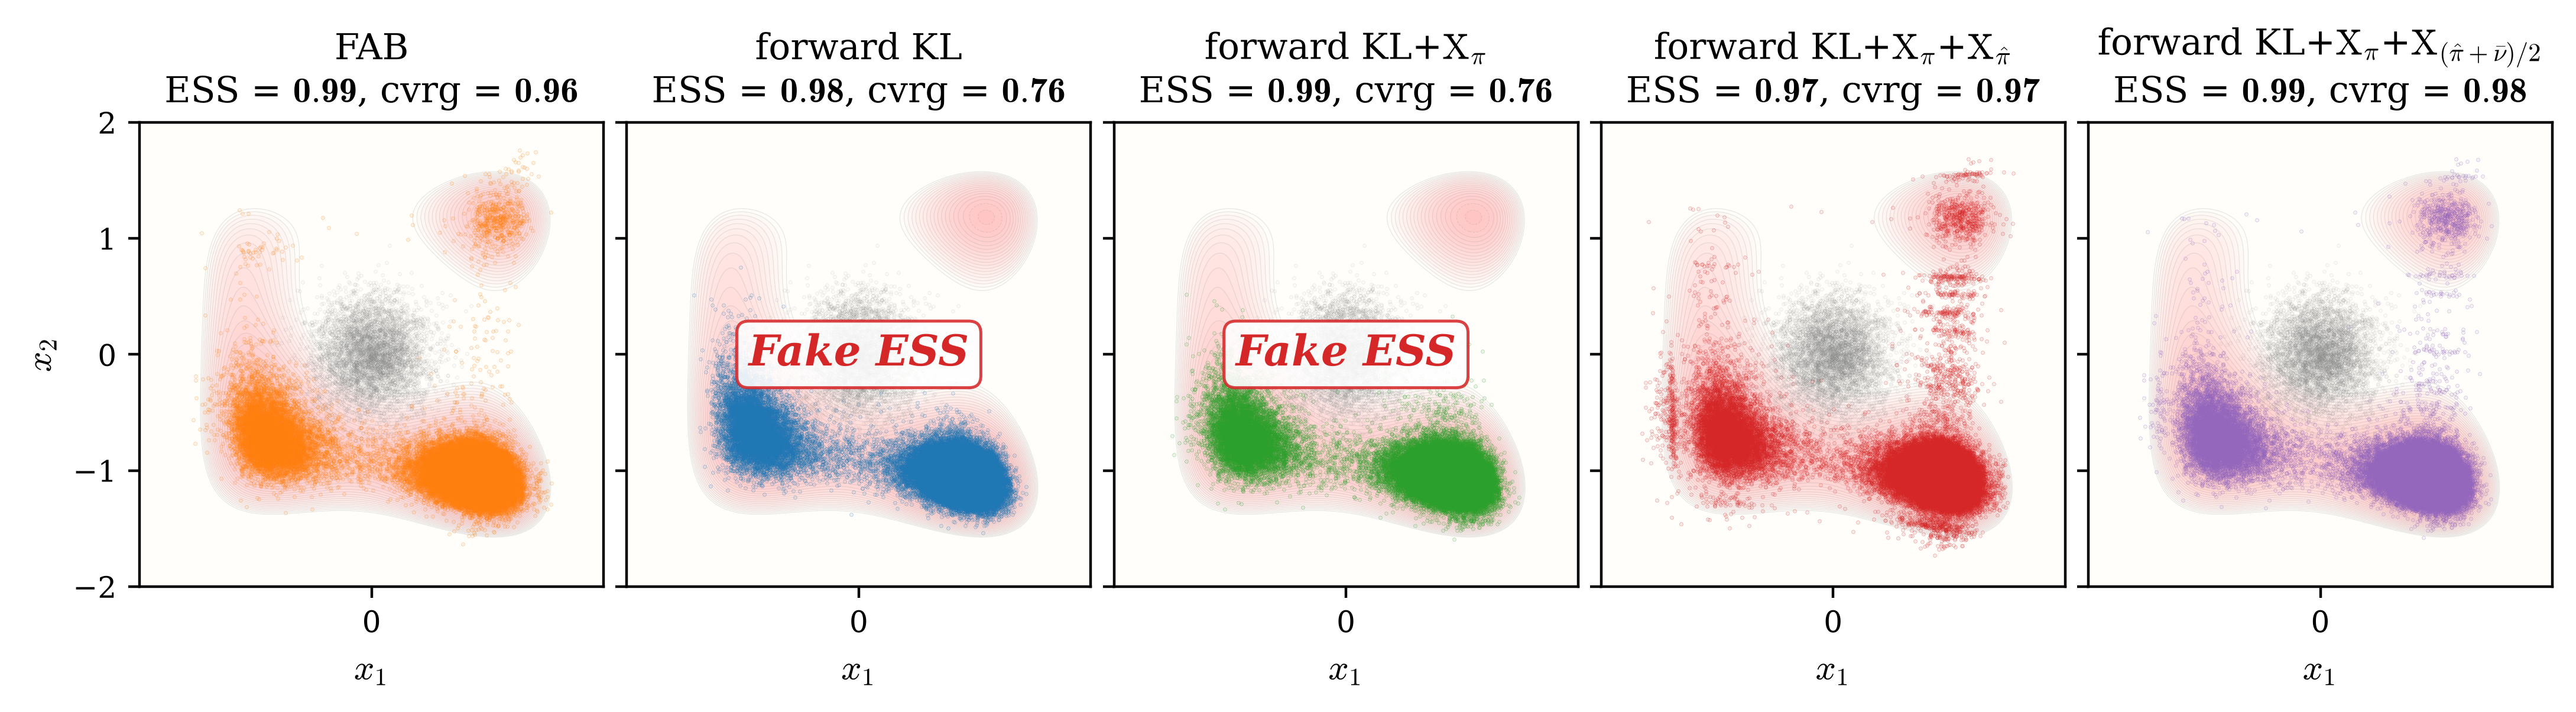
\includegraphics[width=\textwidth]{figures/2d_three_well_fake_ess.png}\\[3pt]
		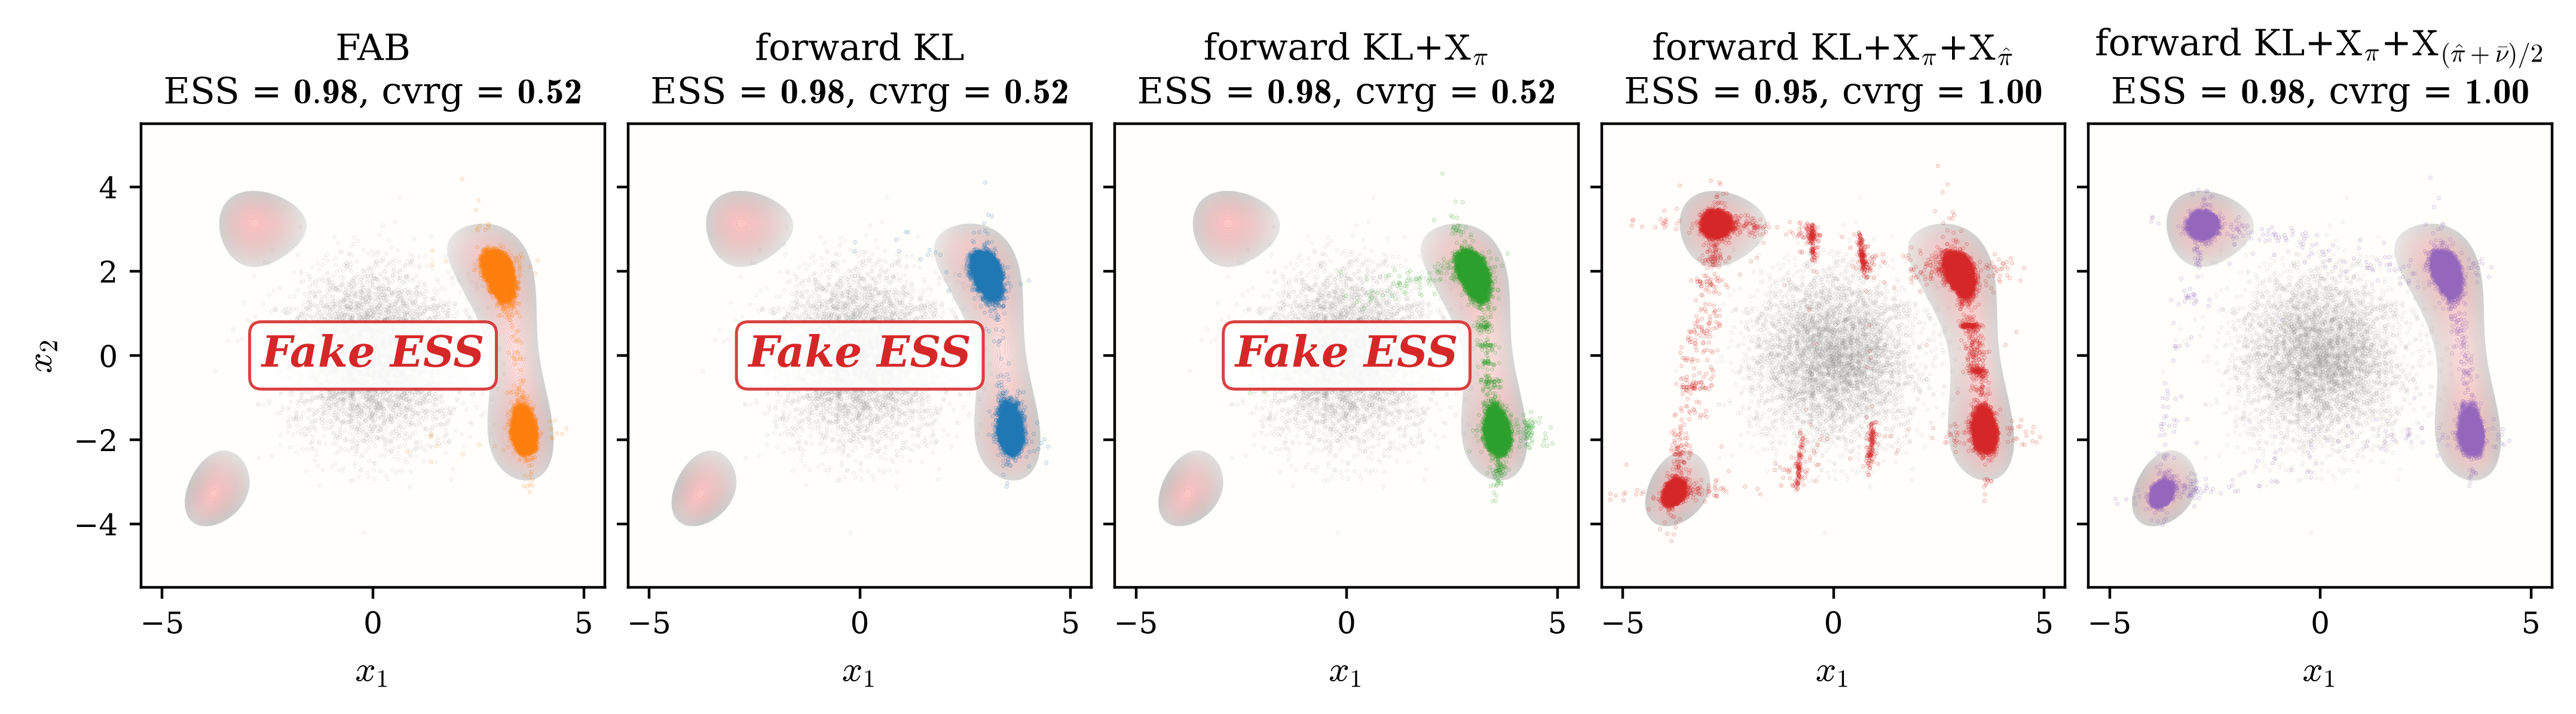
\includegraphics[width=\textwidth]{figures/2d_himmelblau_fake_ess.png}
	\end{center}
	\vspace{-2pt}
	\centering
	Coverage below $0.9$: the ESS is earned only on the wells reached.
\end{frame}

\begin{frame}{Product Multi-Well up to $d=256$}
	\small
	$U(\bm x) = \tfrac12\lVert\bm x\rVert^2 + 12\sum_{i=1}^{k}e^{-x_i^2}$, $k=\lfloor\log_2 d\rfloor$, $d = 16,\dots,256$.
	\begin{itemize}
		\setlength{\itemsep}{0pt}
		\item KL+L1: log-dispersion regularization penalty LDR-L1 (Schopmans et al.)
		\item FAB: flow annealed importance sampling bootstrap (Midgley et al.)
	\end{itemize}
	\begin{center}
		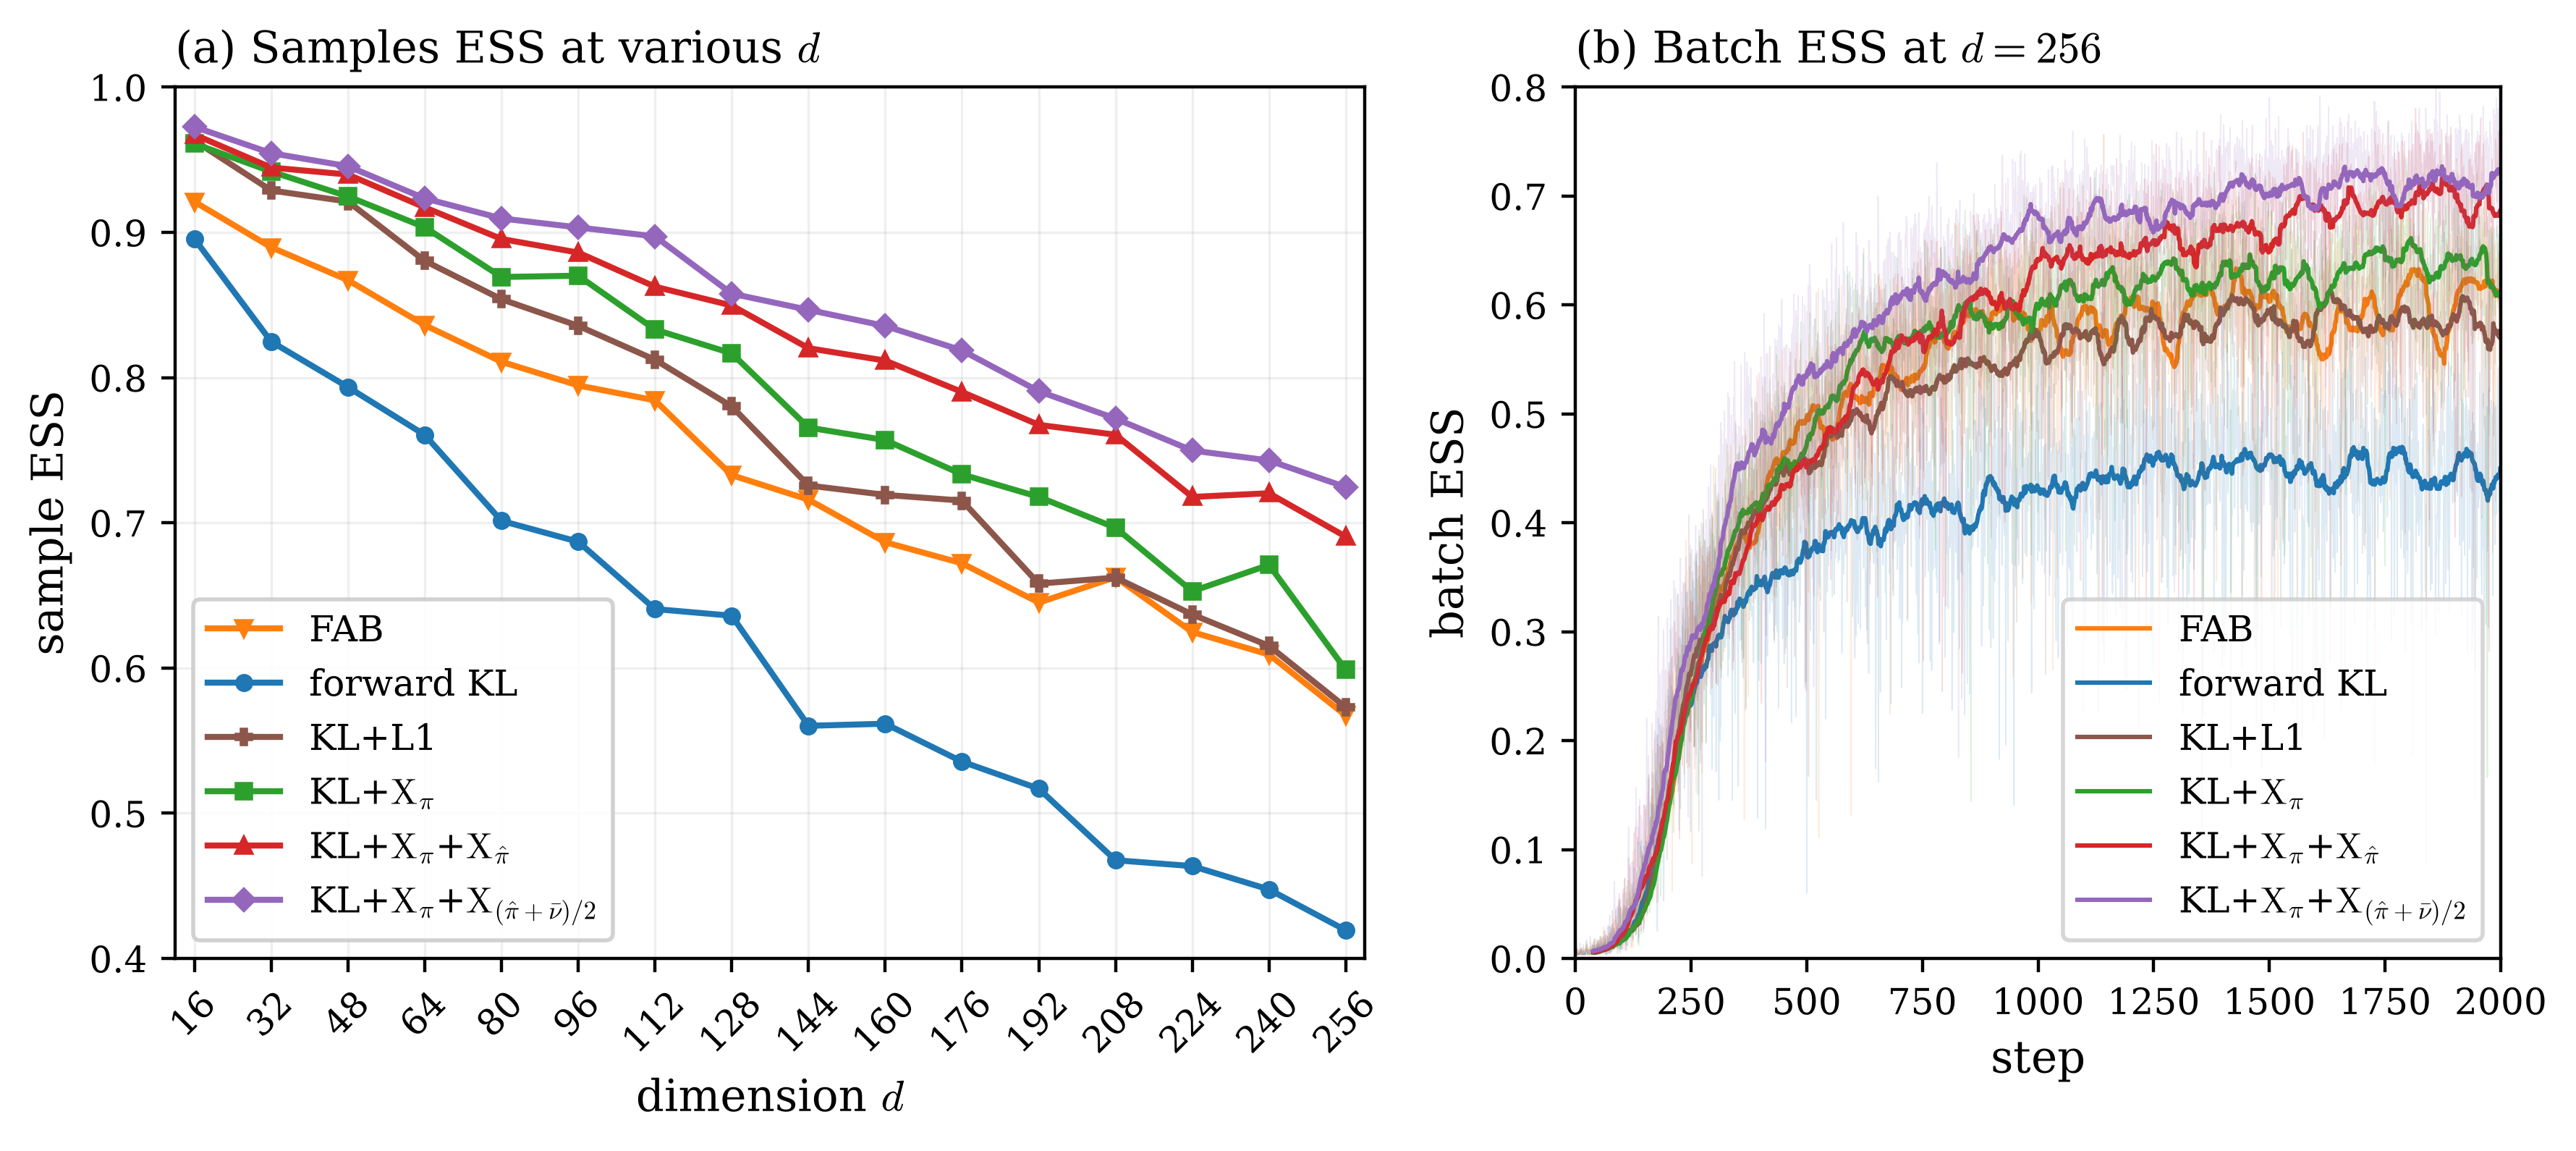
\includegraphics[width=0.88\textwidth]{figures/hd_product_ess.png}
	\end{center}
	\vspace{-0.1cm}
	Every log-ratio variation beats forward KL at all sixteen $d$.
\end{frame}

\begin{frame}{Coefficient Sweep at $d=100$}
	\small
	$\KL$+$\lambda\X_\pi$ on the same potential, $\lambda=0$ being forward KL.
	\begin{center}
		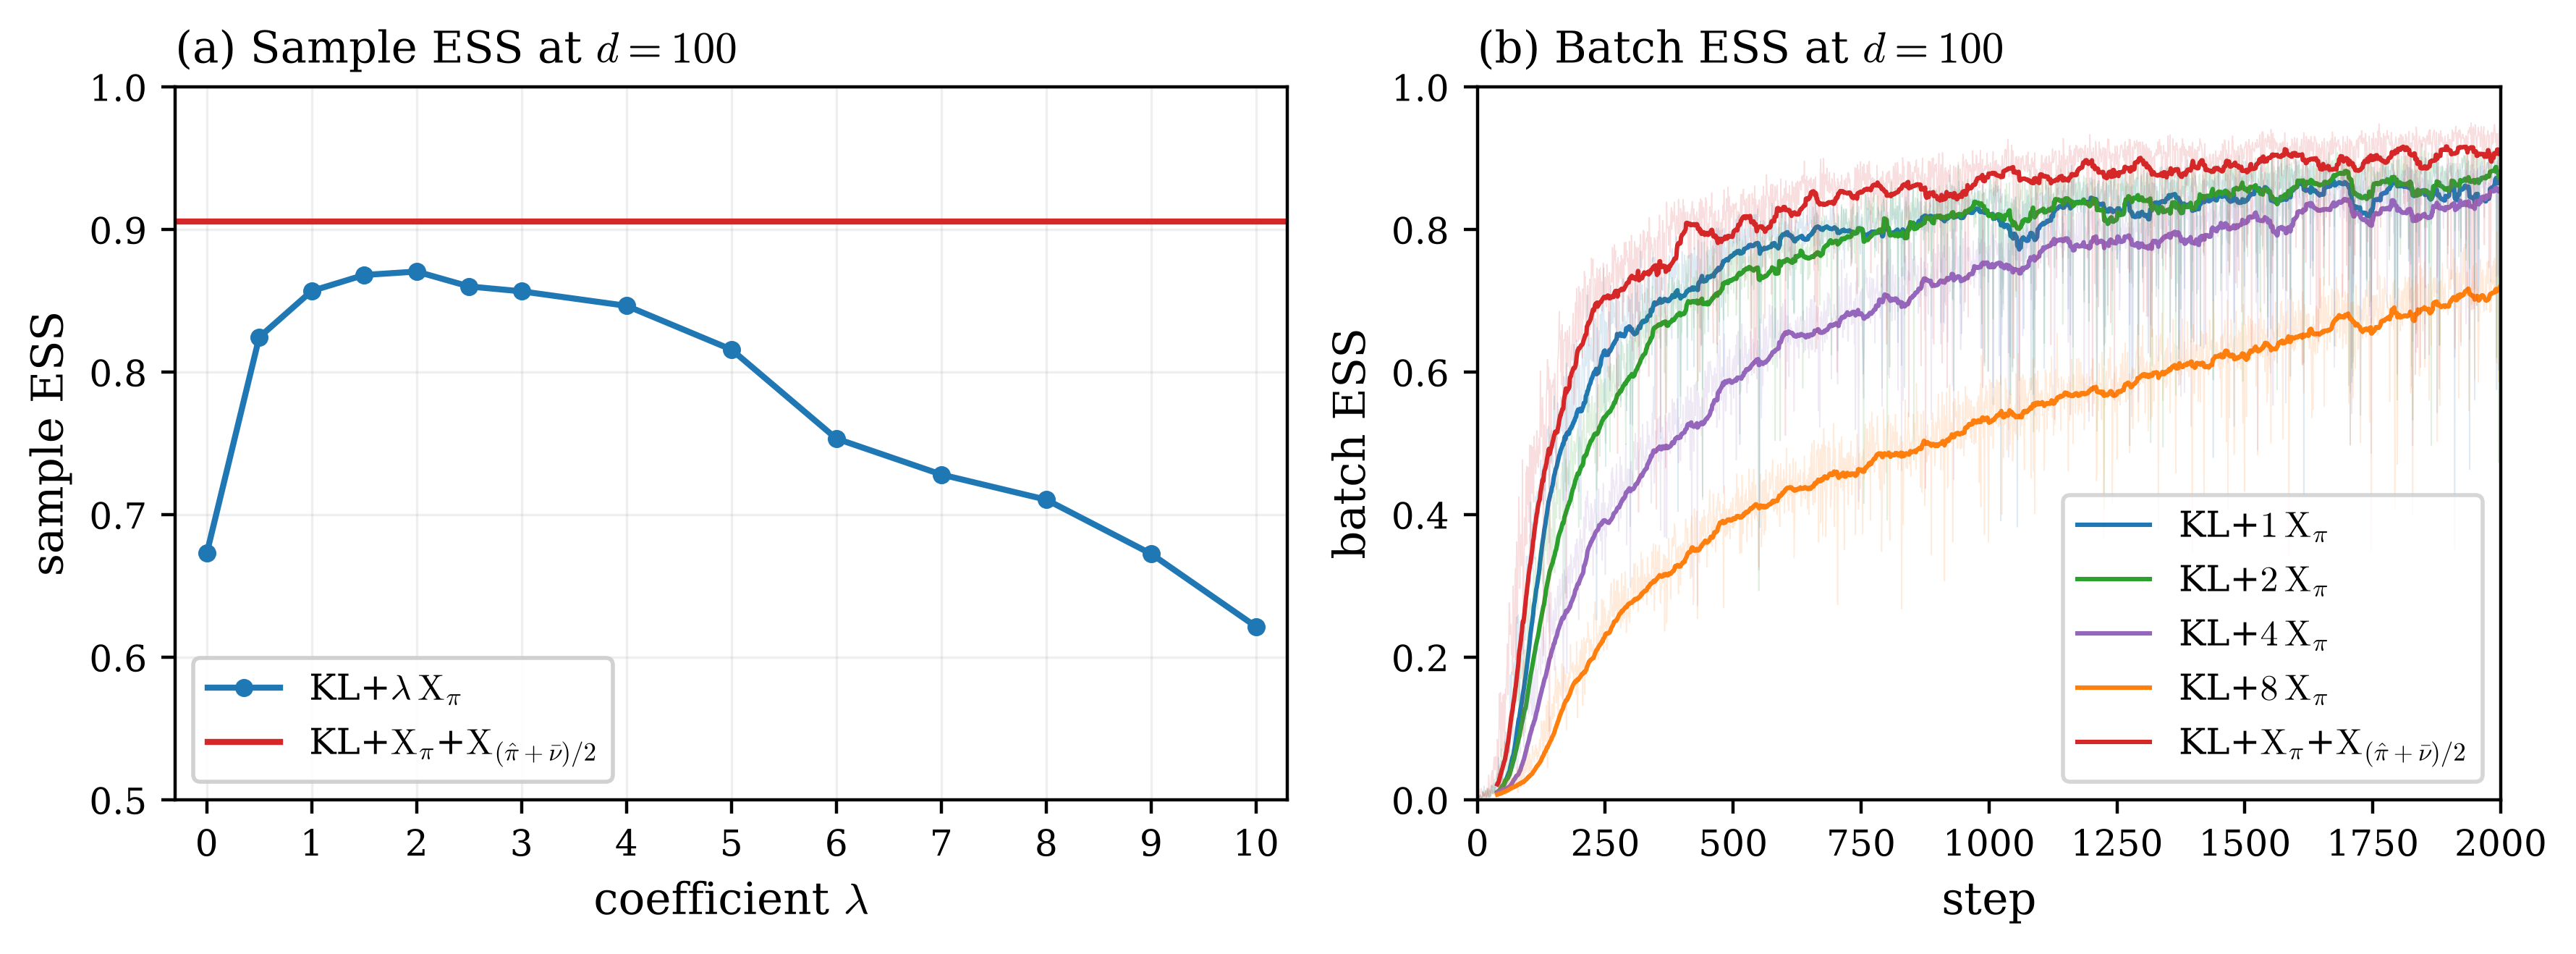
\includegraphics[width=0.88\textwidth]{figures/hd_100_lambda_ess.png}
	\end{center}
	 KLXX ($0.906$, red line) sits above every value the sweep attains. Tuning one coefficient does not reproduce the mixture variation.
\end{frame}

\begin{frame}{Lattice $\phi^4$: a Collective Barrier}
	\small
	Tilted scalar $\phi^4$ action on a periodic $L\times L$ lattice, $d=L^2$, at $L=6$, $h=0.0257$:
	\begin{equation*}
		U(\bm\phi) = -0.8\sum_{\langle jl\rangle}\phi_j\phi_l
		+ \sum_{j=1}^{d}\Bigl[\phi_j^2+\tfrac12(\phi_j^2-1)^2\Bigr] + h\sum_{j=1}^{d}\phi_j ,
		\quad
		m(\bm\phi) = \frac1d\sum_{j=1}^{d}\phi_j .
	\end{equation*}
	A domain-wall barrier separates the two wells; the minority weight $p_+=\mathbb P(m>0)$ must be learned. Only $\hat\pi$-based losses recover the minority weight.
	\begin{center}
		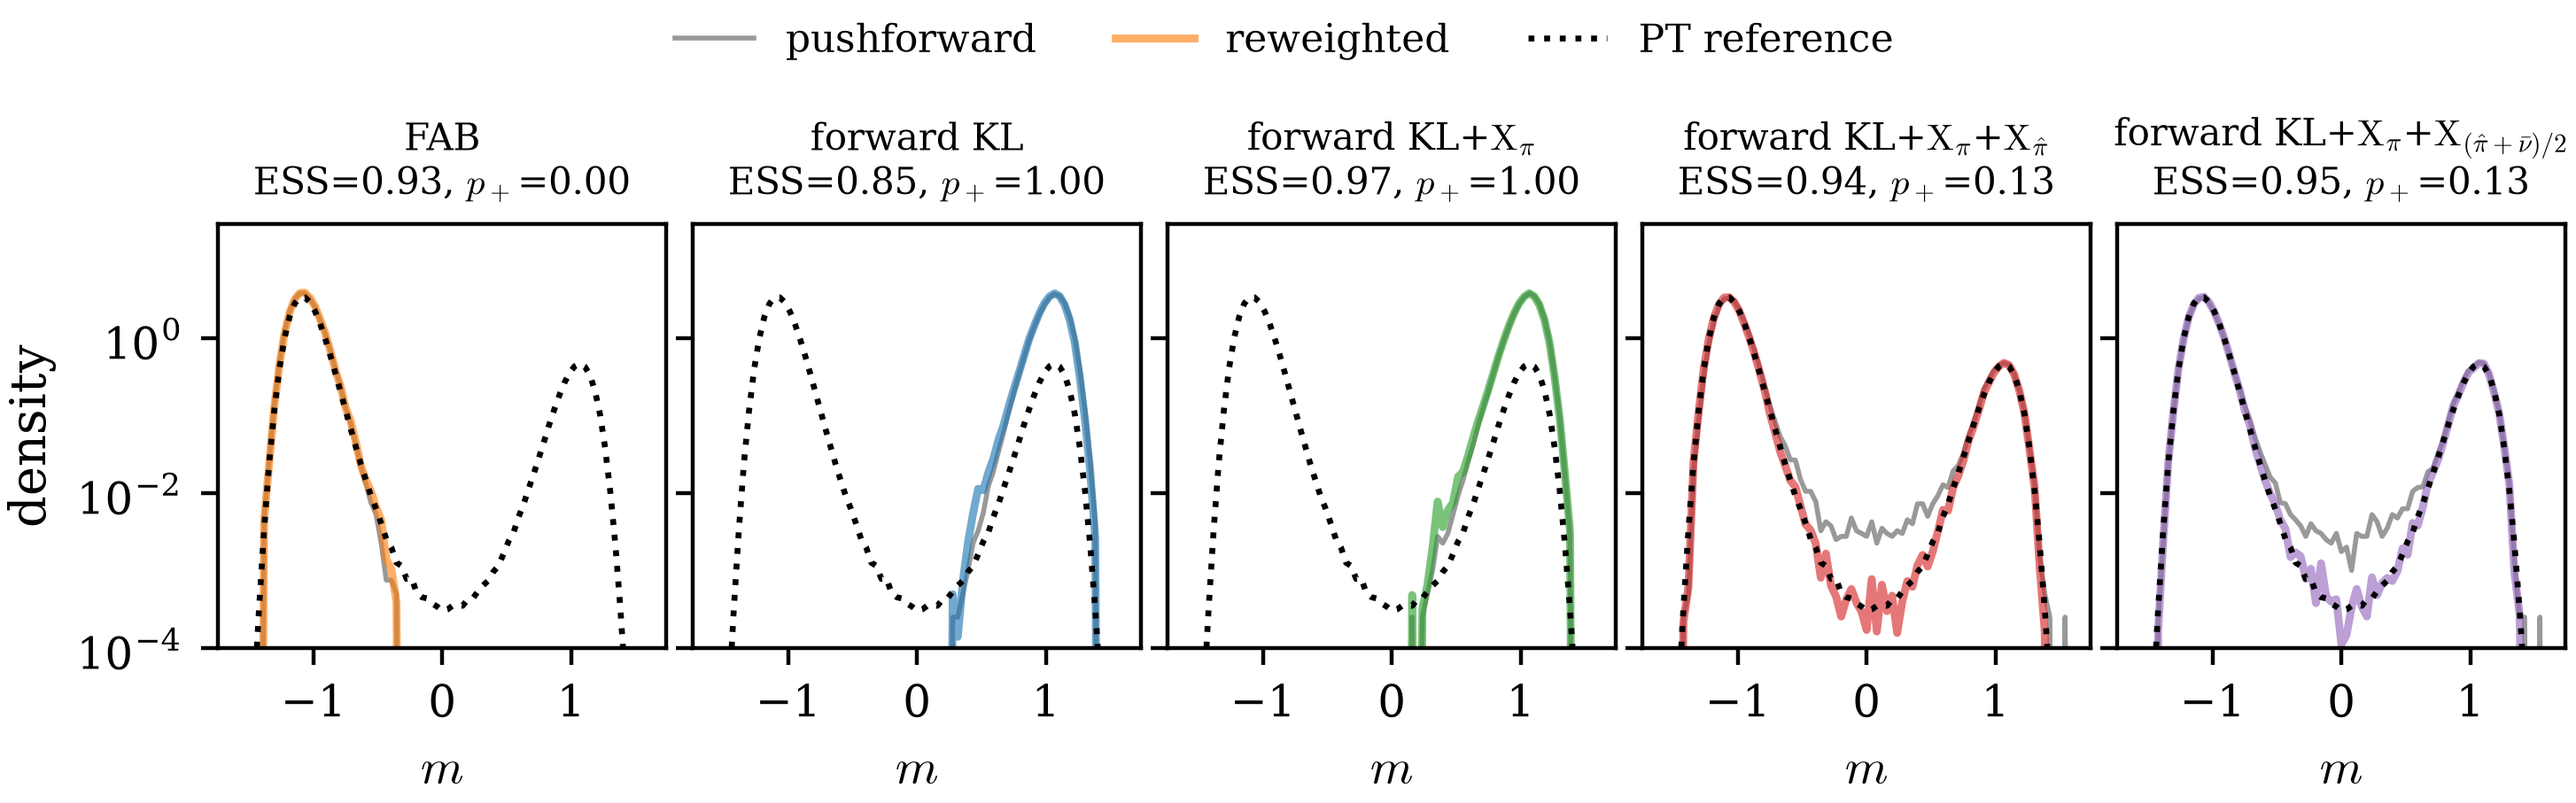
\includegraphics[width=\textwidth]{figures/lattice_phi4_l6_methods.png}
	\end{center}
\end{frame}


\begin{frame}{Boltzmann Generator on Three Molecules}
	\small
	\begin{itemize}
		\setlength{\itemsep}{2pt}
		\item The difficulty is not multimodality alone: the Lennard--Jones core is {\red singular}, so an early proposal can land at energies far outside the thermally occupied region.
		\item Implicit solvent at $300\,\mathrm K$, no target data, one seed. The path is regularized, ending short of the bare potential.
	\end{itemize}
	\vspace{2pt}
	\begin{center}
		\begin{tabular}{lcccc}
			\hline
			& \multicolumn{2}{c}{$\KL$+$\X_\pi$} & \multicolumn{2}{c}{KLXX} \\
			molecule ($d$) & $\hat F$ & stages & $\hat F$ & stages \\
			\hline
			$N$-methylacetamide, NMA ($30$) & $2.06$ & $6$ & \textbf{1.77} & $5$ \\
			glycerol ($36$) & $3.77$ & $7$ & \textbf{3.28} & $6$ \\
			neutral diethanolamine ($48$) & $19.90$ & $10$ & \textbf{15.84} & $10$ \\
			\hline
		\end{tabular}
	\end{center}
	\vspace{2pt}
	\begin{itemize}
		\setlength{\itemsep}{2pt}
		\item Propagation factor $\hat F=\prod_k\ESS_k^{-1/2}$, from the sample ESS of each accepted stage; smaller is better.
	\end{itemize}
\end{frame}


\begin{frame}{Dihedral Marginals against Parallel Tempering}
	\small
	Reference: parallel tempering, six replicas from $300$ to $800\,\mathrm K$. Densities symmetrized under $\varphi\mapsto-\varphi$, as the achiral targets allow.
	\begin{center}
		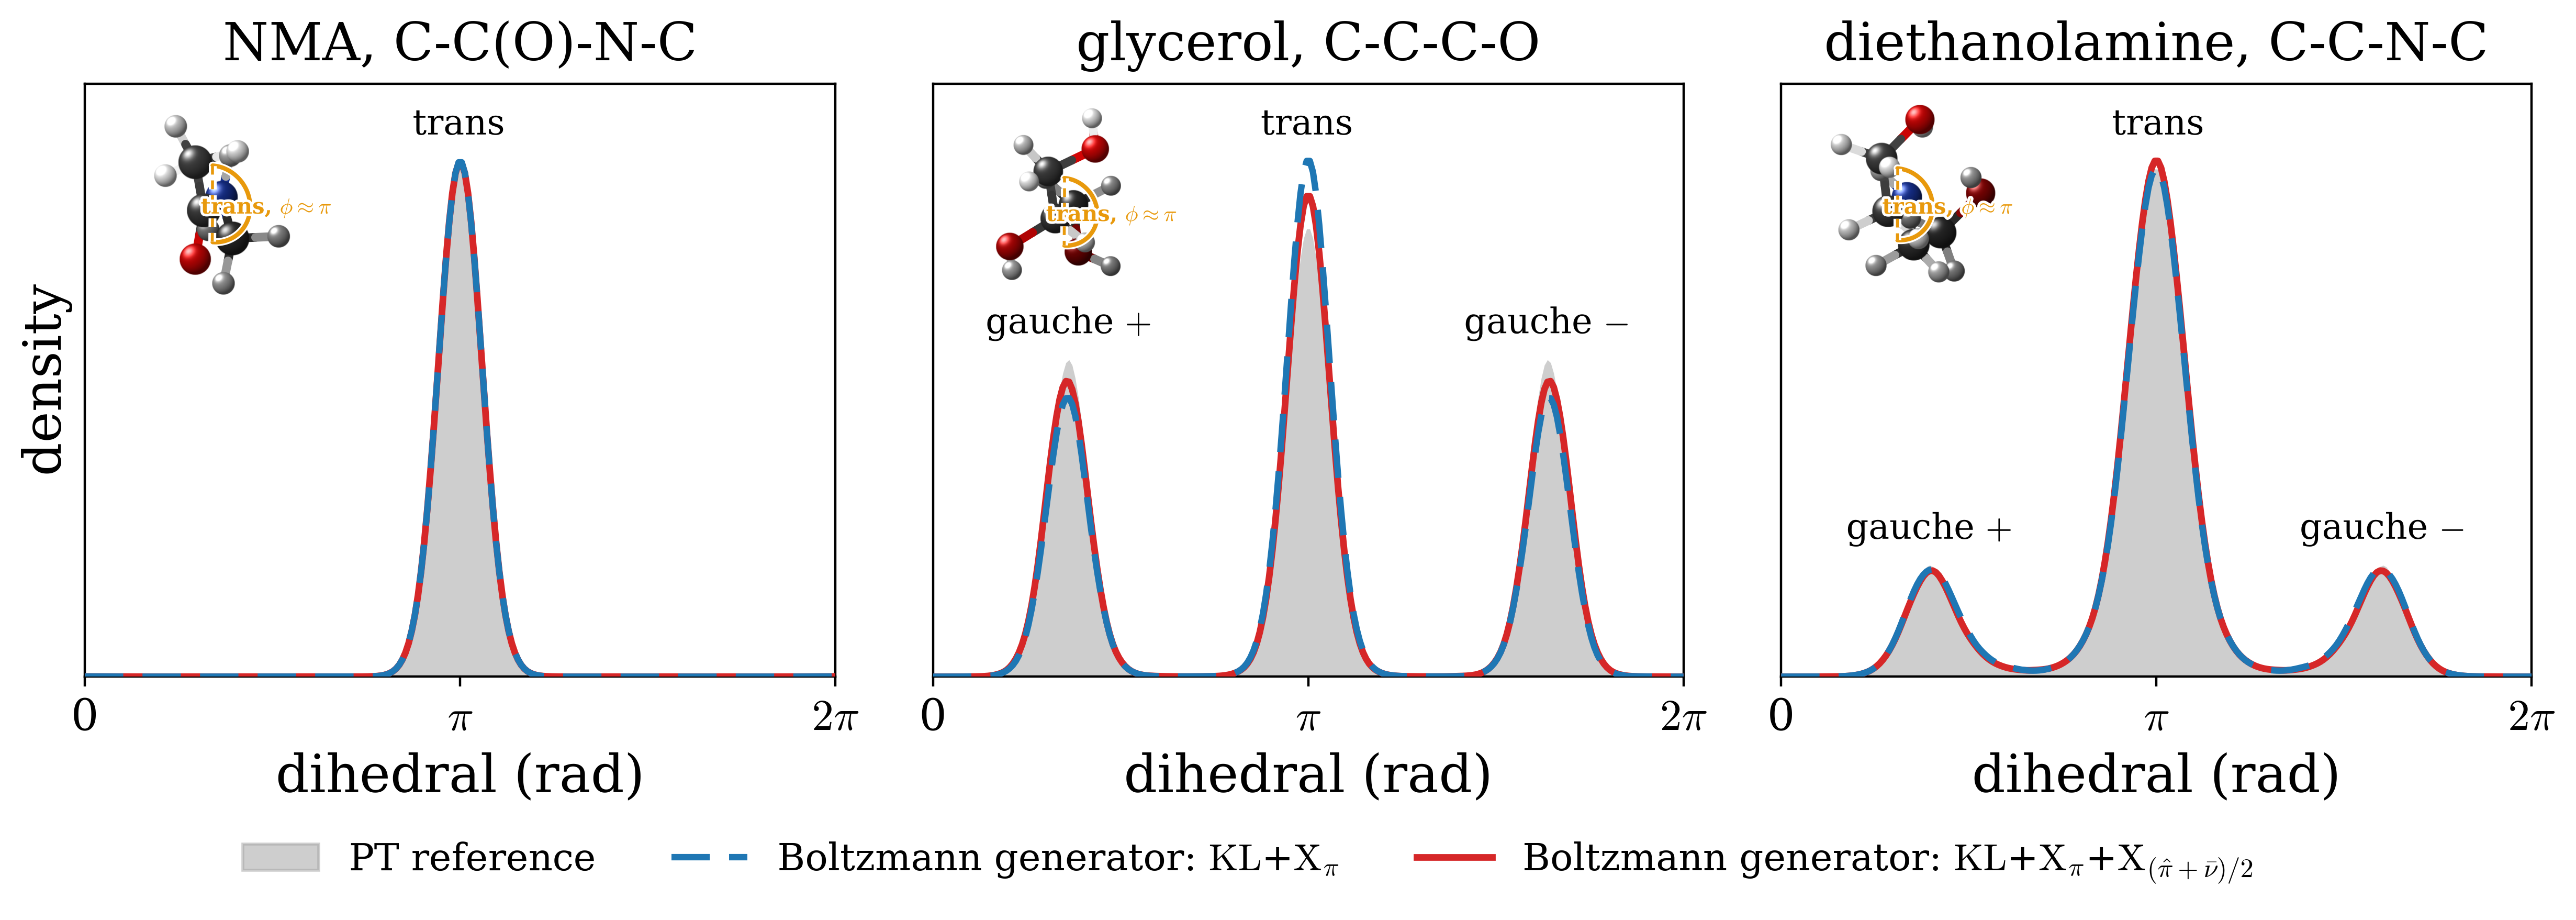
\includegraphics[width=\textwidth]{figures/achiral_dihedrals.png}
	\end{center}
	NMA shows one well: its gauche population is too small to appear. Largest departure: glycerol trans, KLXX at about half of the $\KL$+$\X_\pi$ excess.
\end{frame}



\begin{frame}{Conclusions}
	\small
	\begin{itemize}
		\setlength{\itemsep}{9pt}
		\item Forward KL trains only on the samples it is given. When a mode is missing from the flow and from those samples, the ESS stays high and says nothing: a {\red fake ESS}.
		\item $\X_\omega$ compares $\log(\pi/\nu)$ at pairs of points. It needs no normalizing constant, and it can be evaluated wherever we can draw samples: at $\pi$ for accuracy, at $\hat\pi$ for the modes the flow has not found, at $\bar\nu$ to keep mass out of the gaps.
		\item The loss itself makes the flow {\red visit every mode}. The extra cost per step is two sorts and one more batch, plus the QT set built once.
	\end{itemize}
\end{frame}

\begin{frame}{References}
	\footnotesize
	\begin{itemize}
		\setlength{\itemsep}{5pt}
		\item F. No\'e, S. Olsson, J. K\"ohler, H. Wu. Boltzmann generators. \textit{Science} 365 (2019).
		\item L. Midgley, V. Stimper, G. Simm, B. Sch\"olkopf, J. Hern\'andez-Lobato. Flow annealed importance sampling bootstrap. \textit{ICLR} (2023).
		\item H. Schopmans, C. von Klitzing, P. Friederich. Efficient training of Boltzmann generators using off-policy log-dispersion regularization. arXiv:2602.03729 (2026).
		\item C. Durkan, A. Bekasov, I. Murray, G. Papamakarios. Neural spline flows. \textit{NeurIPS} (2019). The architecture used at every stage here.
	\end{itemize}
\end{frame}



\end{document}
